\chapter{Métodos semânticos de dedução na lógica proposicional}


Capítulo 4 de Souza, \textit{Lógica para Ciência da Computação}~\cite{souza_logica_3}.

\vspace{1cm}


%%%%%%%%%%%%%%%%%%%%%%%%%%%%%%%%%%%%%%%%%%%%%%%%%%%%%%%%%%%%
\section{Introdução}

\begin{easylist}
  & Validade de fórmulas: uma fórmula é válida sse todas as suas interpretações são iguais a $T$.
\end{easylist}


%%%%%%%%%%%%%%%%%%%%%%%%%%%%%%%%%%%%%%%%%%%%%%%%%%%%%%%%%%%%
\section{Método da tabela verdade}

\begin{easylist}
  & Método da tabela verdade: é um método exaustivo, ou seja, enumera todas as possibilidades. A desvantagem é que, se houver muitos símbolos proposicionais, a tabela fica muito grande.
  & Exemplo: seja $H = \; \NOT(P \AND Q) \BIC (\NOT P \OR \NOT Q)$, demonstre que $H$ é uma tautologia usando o método da tabela verdade.  
\end{easylist}

\begin{center}
  \begin{tabular}{ c|c|c|c|c|c|c|c }
    $P$ & $Q$ & $\NOT P$ & $\NOT Q$ & $(P \AND Q)$ & $\NOT(P \AND Q)$ & $(\NOT P \OR \NOT Q)$ & $H$ \\
    \hline
    $T$ & $T$ & $F$      & $F$      & $T$          & $F$              & $F$                   & $T$ \\
    $T$ & $F$ & $F$      & $T$      & $F$          & $T$              & $T$                   & $T$ \\
    $F$ & $T$ & $T$      & $F$      & $F$          & $T$              & $T$                   & $T$ \\
    $F$ & $F$ & $T$      & $T$      & $F$          & $T$              & $T$                   & $T$ \\
  \end{tabular}
\end{center}

%%%%%%%%%%%%%%%%%%%%%%%%%%%%%%%%%%%%%%%%%%%%%%%%%%%%%%%%%%%%
\section{Método da negação ou absurdo}

\begin{easylist}
  & Método da negação ou absurdo: funciona da seguinte maneira.
  && Faça uma suposição.
  && Se todas as substituições possíveis levarem a contradições, a suposição é falsa. Ou seja, a negação da suposição é verdadeira.

  & Exemplo: seja $H = \; ((P \IMP Q) \AND (Q \IMP R)) \IMP (P \IMP R)$, demonstre por absurdo que $H$ é uma tautologia.
  && Demonstração: assuma por absurdo que existe interpretação $I$ tal que $I(H) = F$.

  Então $I((P \IMP Q) \AND (Q \IMP R)) = T$ e
  $I(P \IMP R) = F$.

  Como $I(P \IMP R) = F$, então $I(P) = T$ e $I(R) = F$.

  Distribuindo na fórmula os valores de verdade encontados, temos

$    (( P \IMP Q) \AND (Q \IMP R)) \IMP (P \IMP R)    $

$ \;\;\;    T \hspace{30pt} T \hspace{30pt} F \hspace{10pt} F \;\;\; T \; F \; F  $

de onde obtemos

$    (( P \IMP Q) \AND (Q \IMP R)) \IMP (P \IMP R)    $

$ \;\;\;    T \;\; T \; T \;\; T \;\; F \;\; T \;\; F \hspace{10pt} F \;\;\; T \; F \; F  $

$ \hspace{32pt} \uparrow \hspace{21pt} \uparrow $

\hspace{27pt} Absurdo

Portanto, a suposição inicial de que existe interpretação $I$ tal que $I(H) = F$ é falsa. Em outras palavras, para todo $I$, $I(H)=T$, ou seja, $H$ é tautologia.

  & Exemplo: seja $H = \; (P \IMP Q) \AND ( \NOT( \NOT P \OR Q))$, demonstre por absurdo que $H$ é uma contradição.
  && Demonstração: assuma por absurdo que existe interpretação $I$ tal que $I(H) = T$.

  Então $I(P \IMP Q) = T$ e $I( \NOT( \NOT P \OR Q) ) = T$.

  Como $I( \NOT( \NOT P \OR Q) ) = T$, então $I( \NOT P \OR Q) = F$. E portanto, $I(Q) = F$, $I(\NOT P) = F$ e $I(P) = T$.

  Distribuindo na fórmula os valores de verdade encontados, temos

$    (P \IMP Q) \AND ( \NOT( \NOT P \OR Q))    $

$ \;\;\;\;\;\;    T \hspace{20pt}                   T \;\;\; T \;\;  F \;\;  T \;\;  F \;\;  F  $

mas se $I(P) = T$, temos que $I(Q)$ precisa ser $T$ já que $I(P \IMP Q) = T$, portanto obtemos

$    (P \IMP Q) \AND ( \NOT( \NOT P \OR Q))    $

$ \; T \;\;  T \;\; T \;\;\;                      T \;\;\; T \;\;  F \;\;  T \;\;  F \;\;  F  $

$ \hspace{30pt} \uparrow \hspace{78pt} \uparrow $

\hspace{50pt} Absurdo

Portanto, a suposição inicial de que existe interpretação $I$ tal que $I(H) = T$ é falsa. Em outras palavras, para todo $I$, $I(H)=F$, ou seja, $H$ é contradição.

  & Observe que para demonstrar corretamente que uma fórmula $H$ é tautologia, é necessário chegar a um absurdo em todas as substituições possíveis. Caso alguma substituição não chegue a um absurdo, pode-se interromper a demonstração e concluir que a fórmula não é tautologia. Isso é evidente, pois, se você assume que $I(H) = F$ e não chega a um absurdo, significa que essa substituição específica faz com que $I(H)$ seja $F$ e, portanto, com que $H$ não seja tautologia. Diferentes substituições representam diferentes linhas da tabela verdade, e pode ocorrer de algumas linhas serem iguais a $T$, caso em que há absurdo, e outras linhas iguais a $F$, caso em que não há absurdo. Por isso é necessário explorar todas as substituições possíveis.  O mesmo vale para a contradição.



\end{easylist}


%%%%%%%%%%%%%%%%%%%%%%%%%%%%%%%%%%%%%%%%%%%%%%%%%%%%%%%%%%%%
\section{Método da árvore semântica}

\begin{easylist}
  & Método da árvore semântica: é um método que permite a verificação da validade de uma fórmula sem ser exaustivo. A depender da fórmula, pode ser possível obter a resposta sem verificar todas as interpretações possíveis. Este conteúdo está na primeira edição do livro de Souza \textit{Lógica para Ciência da Computação}~\cite{souza_logica_1}.

%\clearpage
  
  & Exemplo: seja $H = \; \NOT(P \AND Q) \BIC (\NOT P \OR \NOT Q)$, demonstre que $H$ é uma tautologia usando o método da árvore semântica.
\end{easylist}

\begin{center}
  \begin{tabular}{ c|cccccccccc }
        & $\NOT$ & $(P$ & $\AND$ & $Q)$ & $\BIC$ & $(\NOT$ & $P$ & $\OR$ & $\NOT$ & $Q)$ \\
    \hline
      2 &        & $T$  &        &      &        & $F$     & $T$ &       &        &      \\
    \hline
      3 & $T$    & $F$  & $F$    &      & $T$    & $T$     & $F$ & $T$   &        &      \\
    \hline
      4 & $F$    & $T$  & $T$    & $T$  & $T$    & $F$     & $T$ & $F$   & $F$    & $T$  \\
    \hline
      5 & $T$    & $T$  & $F$    & $F$  & $T$    & $F$     & $T$ & $T$   & $T$    & $F$  \\
  \end{tabular}
\end{center}

\begin{figure}[h!]
  \begin{center}
    \begin{tabular}{c}
      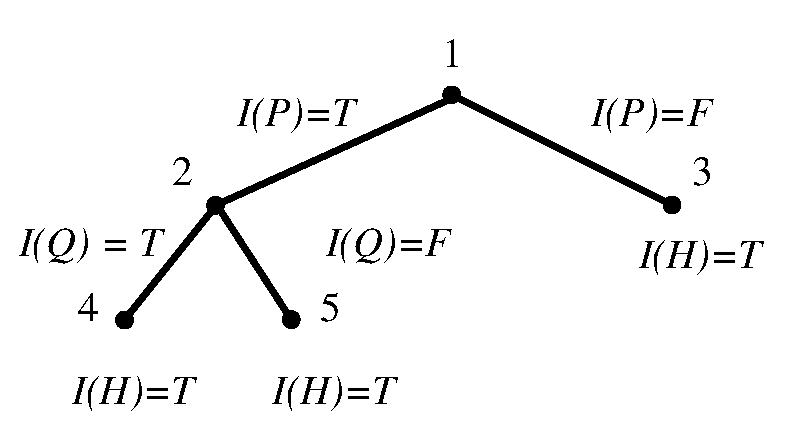
\includegraphics[width=0.7\textwidth]{images/04/tree_01.eps}
    \end{tabular}
  \end{center}
  %\caption{\label{fig:tree:01}}
\end{figure}

\clearpage

\begin{easylist}
  & Exemplo: seja $H = \; (P \OR \NOT Q) \BIC (\NOT P \IMP \NOT Q)$, demonstre que $H$ é uma tautologia usando o método da árvore semântica.
\end{easylist}

\begin{center}
  \begin{tabular}{ c|cccccccccc }
        & $(P$ & $\OR$ & $\NOT$ & $Q)$ & $\BIC$ & $(\NOT$ & $P$ & $\IMP$ & $\NOT$ & $Q)$ \\
    \hline
      2 & $T$  & $T$   &        &      & $T$    & $F$     & $T$ & $T$    &        &      \\
    \hline
      3 & $F$  &       &        &      &        & $T$     & $F$ &        &        &      \\
    \hline
      4 & $F$  & $F$   & $F$    & $T$  & $T$    & $T$     & $F$ & $F$    & $F$    & $T$  \\
    \hline
      5 & $F$  & $T$   & $T$    & $F$  & $T$    & $T$     & $F$ & $T$    & $T$    & $F$  \\
  \end{tabular}
\end{center}

\begin{figure}[h!]
  \begin{center}
    \begin{tabular}{c}
      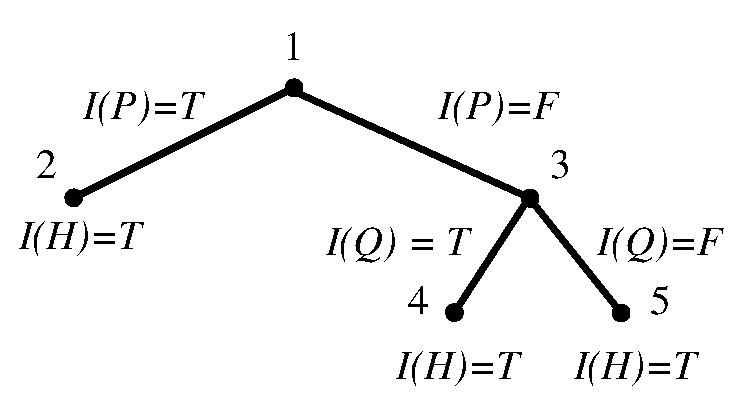
\includegraphics[width=0.7\textwidth]{images/04/tree_02.eps}
    \end{tabular}
  \end{center}
  %\caption{\label{fig:tree:01}}
\end{figure}


%%%%%%%%%%%%%%%%%%%%%%%%%%%%%%%%%%%%%%%%%%%%%%%%%%%%%%%%%%%%
\section{Método dos tableaux semânticos}

\begin{easylist}
  & Tableau semântico: sequência de fórmulas construída de acordo com um conjunto de regras e apresentada em forma de árvore. O método dos tableaux semânticos é um mecanismo de decisão para a pergunta $\beta \vdash H$, sim ou não?

  & Elementos do sistema de tableaux semânticos da lógica proposicional:
  && Alfabeto da lógica proposicional sem os símbolos de verdade $\TRUE$ e $\FALSE$.
  && Conjunto das fórmulas da lógica proposicional.
  && Um conjunto de regras de dedução.

  & Regras de dedução do tableau semântico: sejam $A$ e $B$ duas fórmulas da lógica proposicional, as regras de dedução do sistema de tableaux semânticos são

\clearpage
  
\begin{figure}[h!]
  \begin{center}
    \begin{tabular}{c}
      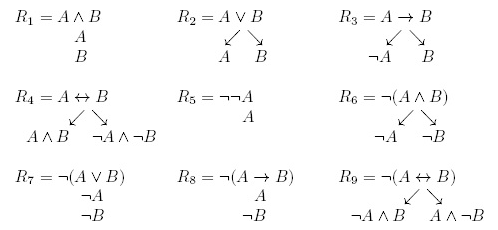
\includegraphics[width=0.7\textwidth]{images/04/tableaux.png}
    \end{tabular}
  \end{center}
  %\caption{\label{fig:tree:01}}
\end{figure}

  & Construção de um tableau semântico: se dá aplicando alguma regra de dedução uma vez para cada linha que não seja um literal (símbolo proposicional ou sua negação). O tableau resultante tende a ficar mais simples se aplicarmos primeiro as regras de dedução que não geram bifurcações $(R_1, R_5, R_7, R_8)$.
&& Exemplo: considere o conjunto de fórmulas $\beta = \{P \OR (Q \OR \NOT R), P \IMP\NOT R, Q \IMP \NOT R\}$. Verifique se $\beta \ISINT \NOT R$.

%$\beta = \{A \IMP B, \NOT(A \OR B),  \NOT (C \IMP A)\}$. Verifique se $\beta \ISINT \NOT R$.

&&& Uma possível solução seria montar a árvore semântica de $\NOT(    (P \OR (Q \OR \NOT R)) \AND (P \IMP\NOT R) \AND (Q \IMP \NOT R)  \IMP \NOT R)$.

%$\NOT (    (  (A \IMP B) \AND \NOT(A \OR B) \AND \NOT (C \IMP A)  ) \IMP \NOT R    )$.

&&& Uma solução equivalente é listar as hipóteses de $\beta$ seguidas da negação da conclusão.
%Encontre o tableau semântico iniciado com esse conjunto de fórmulas.

\end{easylist}

%\forestset{%
%  vertical/.style={                       %define style for phantom node
                                          %with vertical edge drawn from it
%    before drawing tree={not ignore edge, edge=draw},
%  },
%}

%\begin{tableau}
%  {line no sep= 1.5cm,
%    just sep= 1.5cm,
%    for tree={s sep'=10mm},
%    close with=\absurd
%}
%  [((P \land Q) \lor R),                   just={Premiss}
%    [\neg\neg(\neg P \lor \neg R),       just={Negated conclusion}
%      [(\neg P \lor \neg R),           just={From (2)}
%        [(P \land Q),                just={Alternatives from (1)}
%          [P,                      just={From (4)}
%            [Q,                  just={From (4)}
%              [\neg P,close]
%              [\neg R,         just={Alternatives from (3)}
%        ]]]]
%        [R
%          [, vertical               %phantom node but with edge
%            [, vertical       %phantom node but with edge
%              [\neg P]          %and now we have two
%              [\neg R,close]    %brances added
%  ]]]]]]
%\end{tableau}

\iffalse

\forestset{%
  vertical/.style={     %define style for phantom node
                        %with vertical edge drawn from it
    before drawing tree={not ignore edge, edge=draw},
  },
}

\begin{tableau}
{                              % begin tree preamble
    line no sep= 2cm,          % distance of tree from line numbers
    just sep= 1.5cm,
    for tree={s sep'=10mm},    % control horizontal spread of branches
}                              % end tree preamble
  [P
    [(P \IMP Q)                just={From 1.}
      [\NOT Q                  just={From 1.}
        [\NOT P, close]        just={From 1.}
        [Q, close]             just={From 1.}
      ]                        just={From 1.}
    ]                          just={From 1.}
  ]
\end{tableau}

\fi


\begin{prooftree}
  {
    to prove={\{P \OR (Q \OR \NOT R), P \IMP\NOT R, Q \IMP \NOT R\}
      \vdash{}{} \NOT R}
  }
  [P \OR (Q \OR \NOT R), just=Hip, checked
    [P \IMP \NOT R, just=Hip, checked
      [Q \IMP \NOT R, just=Hip, checked,name=last premise
        [\NOT\NOT R, just={$\NOT$ Conc},name=not conc
          [P, just={$\OR$ Elim:!uuuu}
            [\NOT P, close={:!u,!c}]
            [\NOT R, close={:not conc,!c},just={$\IMP$ Elim:!uuuu}]
          ]
          [Q \OR \NOT R
            [Q, move by=1
              [\NOT Q, close={:!u,!c}]
              [\NOT R, close={:not conc,!c},just={$\IMP$ Elim:last premise}]
            ]
            [\NOT R, close={:not conc,!c},move by=1, just={$\OR$ Elim:!u}]
          ]
        ]
      ]
    ]
  ]
\end{prooftree}



\clearpage

\begin{easylist}

& Ramo: é uma sequência de fórmulas onde cada fórmula é derivada das anteriores através das regras de dedução. A primeira fórmula do ramo é sempre a primeira fórmula do tableau.

& Ramo saturado: é um ramo onde, para todas as suas fórmulas,
&& já foi aplicada alguma regra de dedução; ou
&& não é possível aplicar nenhuma regra de derivação, isto é, a fórmula é um literal.

& Ramo fechado: é um ramo que contém uma fórmula e sua negação. Um ramo pode ser fechado sem ser saturado.

& Ramo aberto: é um ramo saturado não fechado.

& Tableau fechado: é um tableau onde todos os ramos são fechados.

& Tableau aberto: é um tableau onde algum ramo é aberto.

& Prova de $H$ no sistema de tableaux semânticos: é um tableau fechado iniciado com a fórmula $\NOT H$
&& Exemplos: verifique se as fórmulas abaixo são tautologias:
&&& $ H_1 = \NOT((P \IMP Q) \AND \NOT (P \BIC Q) \AND \NOT\NOT P) $
&&& $ H_2 = (P \BIC Q) \OR \NOT P $
&&& $ H_3 = (  ( (P \AND Q) \AND (Q \IMP Q_1) ) \AND ( (P \AND Q_1) \IMP \NOT P_1 )  ) \IMP \NOT P_1 $

\end{easylist}

\SKIP


\begin{prooftree}
  {
    to prove={ (  ( (P \AND Q) \AND (Q \IMP Q_1) ) \AND ( (P \AND Q_1) \IMP \NOT P_1 )  ) \IMP \NOT P_1 }
  }
  [\NOT(    (  ( (P \AND Q) \AND (Q \IMP Q_1) ) \AND ( (P \AND Q_1) \IMP \NOT P_1 )  ) \IMP \NOT P_1    ), just=$\NOT H_3$, checked
    [(  ( (P \AND Q) \AND (Q \IMP Q_1) ) \AND ( (P \AND Q_1) \IMP \NOT P_1 )  ), just=$R_8$ em 1, checked
      [\NOT\NOT P_1, just=$R_8$ em 1, checked
        [P_1, just=$R_5$ em 3
          [(P \AND Q) \AND (Q \IMP Q_1), just=$R_1$ em 2, checked
            [(P \AND Q_1) \IMP \NOT P_1, just=$R_1$ em 2, checked
              [P \AND Q, just=$R_1$ em 5, checked
                [Q \IMP Q_1, just=$R_1$ em 5, checked
                  [P, just=$R_1$ em 7
                    [Q, just=$R_1$ em 7
                      [\NOT(P \AND Q_1), just=$R_3$ em 6, checked
                        [\NOT Q, just=$R_3$ em 8
                          [\NOT P, just=$R_6$ em 11,   close={12,10}]
                          [\NOT Q_1, just=$R_6$ em 11, close={12,10}]
                        ]
                        [Q_1,
                          [\NOT P, just=$R_6$ em 11,   close={13,9}]
                          [\NOT Q_1, just=$R_6$ em 11, close={13,12}]
                        ]
                      ]
                      [\NOT P_1
                          [\NOT Q,                    close={11,4}]
                          [Q_1,                       close={11,4}]
                      ]
                    ]
                  ]
                ]
              ]
            ]
          ]
        ]
      ]
    ]
  ]
\end{prooftree}

\SKIP


\begin{easylist}

&&&& Observe que o tableau foi desenvolvido até que todos os ramos ficassem saturados. Alternativamente, é possível fechar os ramos à medida que são encontrados pares de fórmulas contraditórias entre si, como na versão abaixo

\end{easylist}


\begin{prooftree}
  {
    to prove={ (  ( (P \AND Q) \AND (Q \IMP Q_1) ) \AND ( (P \AND Q_1) \IMP \NOT P_1 )  ) \IMP \NOT P_1 }
  }
  [\NOT(    (  ( (P \AND Q) \AND (Q \IMP Q_1) ) \AND ( (P \AND Q_1) \IMP \NOT P_1 )  ) \IMP \NOT P_1    ), just=$\NOT H_3$, checked
    [(  ( (P \AND Q) \AND (Q \IMP Q_1) ) \AND ( (P \AND Q_1) \IMP \NOT P_1 )  ), just=$R_8$ em 1, checked
      [\NOT\NOT P_1, just=$R_8$ em 1, checked
        [P_1, just=$R_5$ em 3
          [(P \AND Q) \AND (Q \IMP Q_1), just=$R_1$ em 2, checked
            [(P \AND Q_1) \IMP \NOT P_1, just=$R_1$ em 2, checked
              [P \AND Q, just=$R_1$ em 5, checked
                [Q \IMP Q_1, just=$R_1$ em 5, checked
                  [P, just=$R_1$ em 7
                    [Q, just=$R_1$ em 7
                      [\NOT(P \AND Q_1), just=$R_3$ em 6, checked
                        [\NOT Q, just=$R_3$ em 8,      close={12,10}]
                        [Q_1,
                          [\NOT P, just=$R_6$ em 11,   close={13,9}]
                          [\NOT Q_1, just=$R_6$ em 11, close={13,12}]
                        ]
                      ]
                      [\NOT P_1,                      close={11,4}]
                    ]
                  ]
                ]
              ]
            ]
          ]
        ]
      ]
    ]
  ]
\end{prooftree}


\begin{easylist}

&& Pergunta: um tableau iniciado com uma tautologia necessariamente terá todos os ramos abertos?
&&& Resposta: não. Um contra-exemplo é a fórmula $ (P \AND \NOT P) \OR (Q \IMP Q) $

& Para provar que uma fórmula $H$ é tautologia, iniciamos um tableau semântico com $\NOT H$, que é uma contradição. Se $H$ for realmente uma tautologia, todas as interpretações de $\NOT H$ devem ser iguais a $F$, fazendo com que todos os ramos do tableau sejam fechados. O método do tableau semântico pode ser visto como uma variação do método da negação ou absurdo, onde ramos fechados correspondem a substituições que levam a um absurdo. Ramos abertos por sua vez correspondem a substituições que não levam a um absurdo, ou seja, substituições que fazem $I(\NOT H) = T$.

\end{easylist}


\subsection{Prova de que uma fórmula é uma contradição}

\begin{easylist}

& Na seção anterior, vimos que é possível mostrar que $H$ é uma tautologia iniciando um tableau semântico com $\NOT H$, que é uma contradição e obtendo um tableau com todos os ramos fechados. Da mesma maneira, é possível mostrar que $H$ é uma contradição iniciando um tableau com $H$ e obtendo um tableau com todos os ramos fechados.  

\end{easylist}


\subsection{Prova de que um conjunto de fórmulas é insatisfatível}

\begin{easylist}

& Como foi visto na seção~\ref{lprop:propriedadesSemanticas}, um conjunto de fórmulas $\beta = \{H_1, H_2, \dots, H_n\}$ é dito insatisfaftível sse não existe interpretação que faça com que todas as fórmulas tenham interpretação igual a $T$ ao mesmo tempo. Em outras palavras, se o conjunto $\beta$ é insatisfatível, podemos dizer que $I(H_1 \AND H_2 \AND \dots \AND H_n) = F$ para toda interpretação, ou seja, essa fórmula é contraditória. É possível então mostrar que o conjunto de fórmulas $\beta$ é insatisfatível através de um tableau semântico fechado iniciado por $H_1 \AND H_2 \AND \dots \AND H_n$.

%Na seção anterior, vimos que é possível mostrar que $H$ é uma tautologia iniciando um tableau semântico com $\NOT H$, que é uma contradição e obtendo um tableau com todos os ramos fechados. Da mesma maneira, é possível mostrar que $H$ é uma contradição iniciando um tableau com $H$ e obtendo um tableau com todos os ramos fechados.  

\end{easylist}




%%%%%%%%%%%%%%%%%%%%%%%%%%%%%%%%%%%%%%%%%%%%%%%%%%%%%%%%%%%%
\section{Exercícios}

%$ \NOT \; \OR \; \AND \; \IMP \; \BIC$

\begin{enumerate}
  \item Determine por absurdo se as fórmulas a seguir são ou não tautologias.
    \begin{enumerate}
      \item $H_1 = (H \OR  H) \IMP H$
      \item $H_2 =  H \IMP (G \OR H)$
      \item $H_3 = (H \IMP G) \IMP ( (E \OR  H) \IMP (G \OR  E) )$
      \item $H_4 = (H \IMP G) \IMP ( (G \IMP E) \IMP (H \IMP E) )$
      \item $H_5 = ( (G \IMP (E \IMP H)) \AND (G \IMP E) ) \IMP (G \IMP H)$
      \item $H_6 = A \IMP ((B \AND C) \IMP ((D \AND E) \IMP ((G \AND H) \IMP A )))$
      \item $H_7 = ((((A \IMP B) \IMP (\NOT C \IMP \; \NOT D)) \IMP C) \IMP E) \IMP \\ ((E \IMP A) \IMP (D \IMP A))$
    \end{enumerate}
  \item Determine por absurdo se as fórmulas a seguir são ou não tautologias.
    \begin{enumerate}
      \item $H_1 = \NOT(\NOT H) \BIC H$
      \item $H_2 = \NOT(H \IMP G) \BIC (\NOT H \BIC G)$
      \item $H_3 = \NOT(H \BIC G) \BIC (\NOT H \BIC G)$
      \item $H_4 = (H \BIC G) \BIC ((H \IMP G) \AND (G \IMP H))$
      \item $H_5 = (H \AND (G \OR E)) \BIC ((H \AND G) \OR (H \AND E))$
      \item $H_6 = ( (H \IMP G) \AND (G \IMP H) ) \IMP (H \IMP H)$
      \item $H_7 = ( (H \BIC G) \AND (G \BIC H) ) \IMP (H \BIC H)$
      \item $H_8 = H \IMP (H \AND G)$
    \end{enumerate}
  \item Repita os exercícios anteriores usando o método do tableau semântico.
\end{enumerate}
